\subsection{Physcis of Proton-Proton Collisions}



A proton is a baryon, it consists of three quarks: $uud$. These three quarks are called valence quarks. They interact with each other by exchanging gluons which can produce virtual $q\bar{q}$ pairs (Fig. \ref{fig:ppCollision}). Such quarks are called sea quarks. \\

%An electric charge of a proton is a sum of the quarks charges: Q=+2/3+2/3-1/3=1. The situation with the mass is different: the mass of a u quark is 6 GeV and the mass of a d quark is 3 GeV while the mass of a proton is 940 GeV. The mass of a proton is an invariant mass of a system of the quarks which is mostly comprised of their kinetic energy. \\

The dymanics of proton interactions depend on the protons energies. If two low energetic protons interact, it corresponds to the large distance between them and such protons do not probe one another's structure. They see each other as colorless electrically charged particles and therefore interact electromagnetically by exchanging a photon. Protons of higher energy see one another's intrinsic structure. Its partons (quarks, antiquarks and gluons) interact strongly with each other.\\

Any parton from one proton can interact with any parton from another proton. QCD describes probabilities of any particular constituent to interact depending on the total momentum transfer and a momentum fraction of a specific parton. These probabilities are called P.D.F. (parton distribution functions). P.D.F. depend on a collider energy and for LHC gluon-gluon interactions have the largest probabilities to occur.\\

However, in W$\gamma$ measurement we are only selecting events with original partons which can produce a W boson. Gluons do not couple directly to a W boson, thus, we are only interested in quark-antiquark pairs which would have a total charge corresponding to the charge of a W boson ($\pm 1$). Since we have $u$ and $d$ as valence quarks and we know that the probability to couple to the same generation quark in charged weak interactions is the highest, most of the W bosons are created by $u\bar{d}$ and $d\bar{u}$ pairs however other $q\bar{q'}$ combinations with the total charges of $\pm 1$ are also possible.\\

\begin{figure}[htb]
  \begin{center}
    {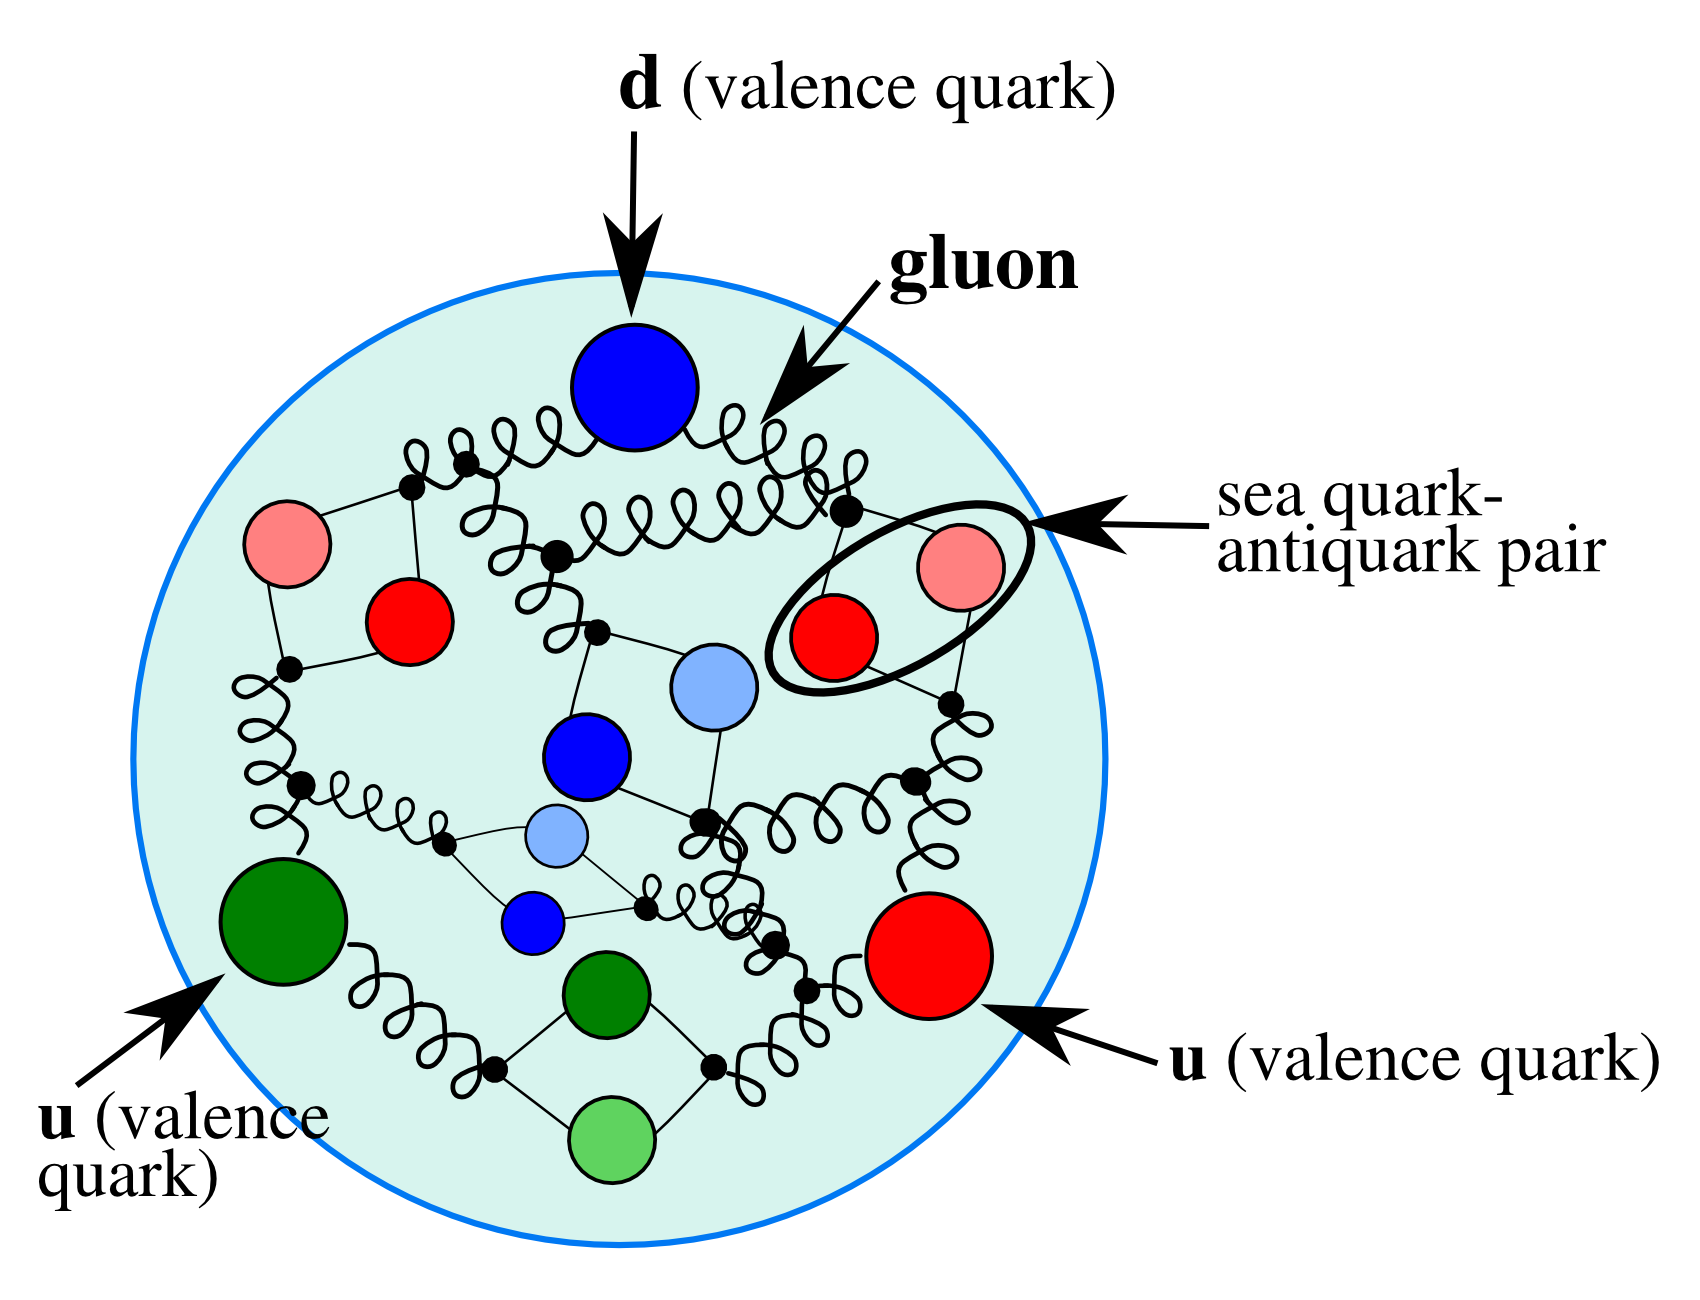
\includegraphics[width=0.45\textwidth]{../figs/Intro/protonStructure.png}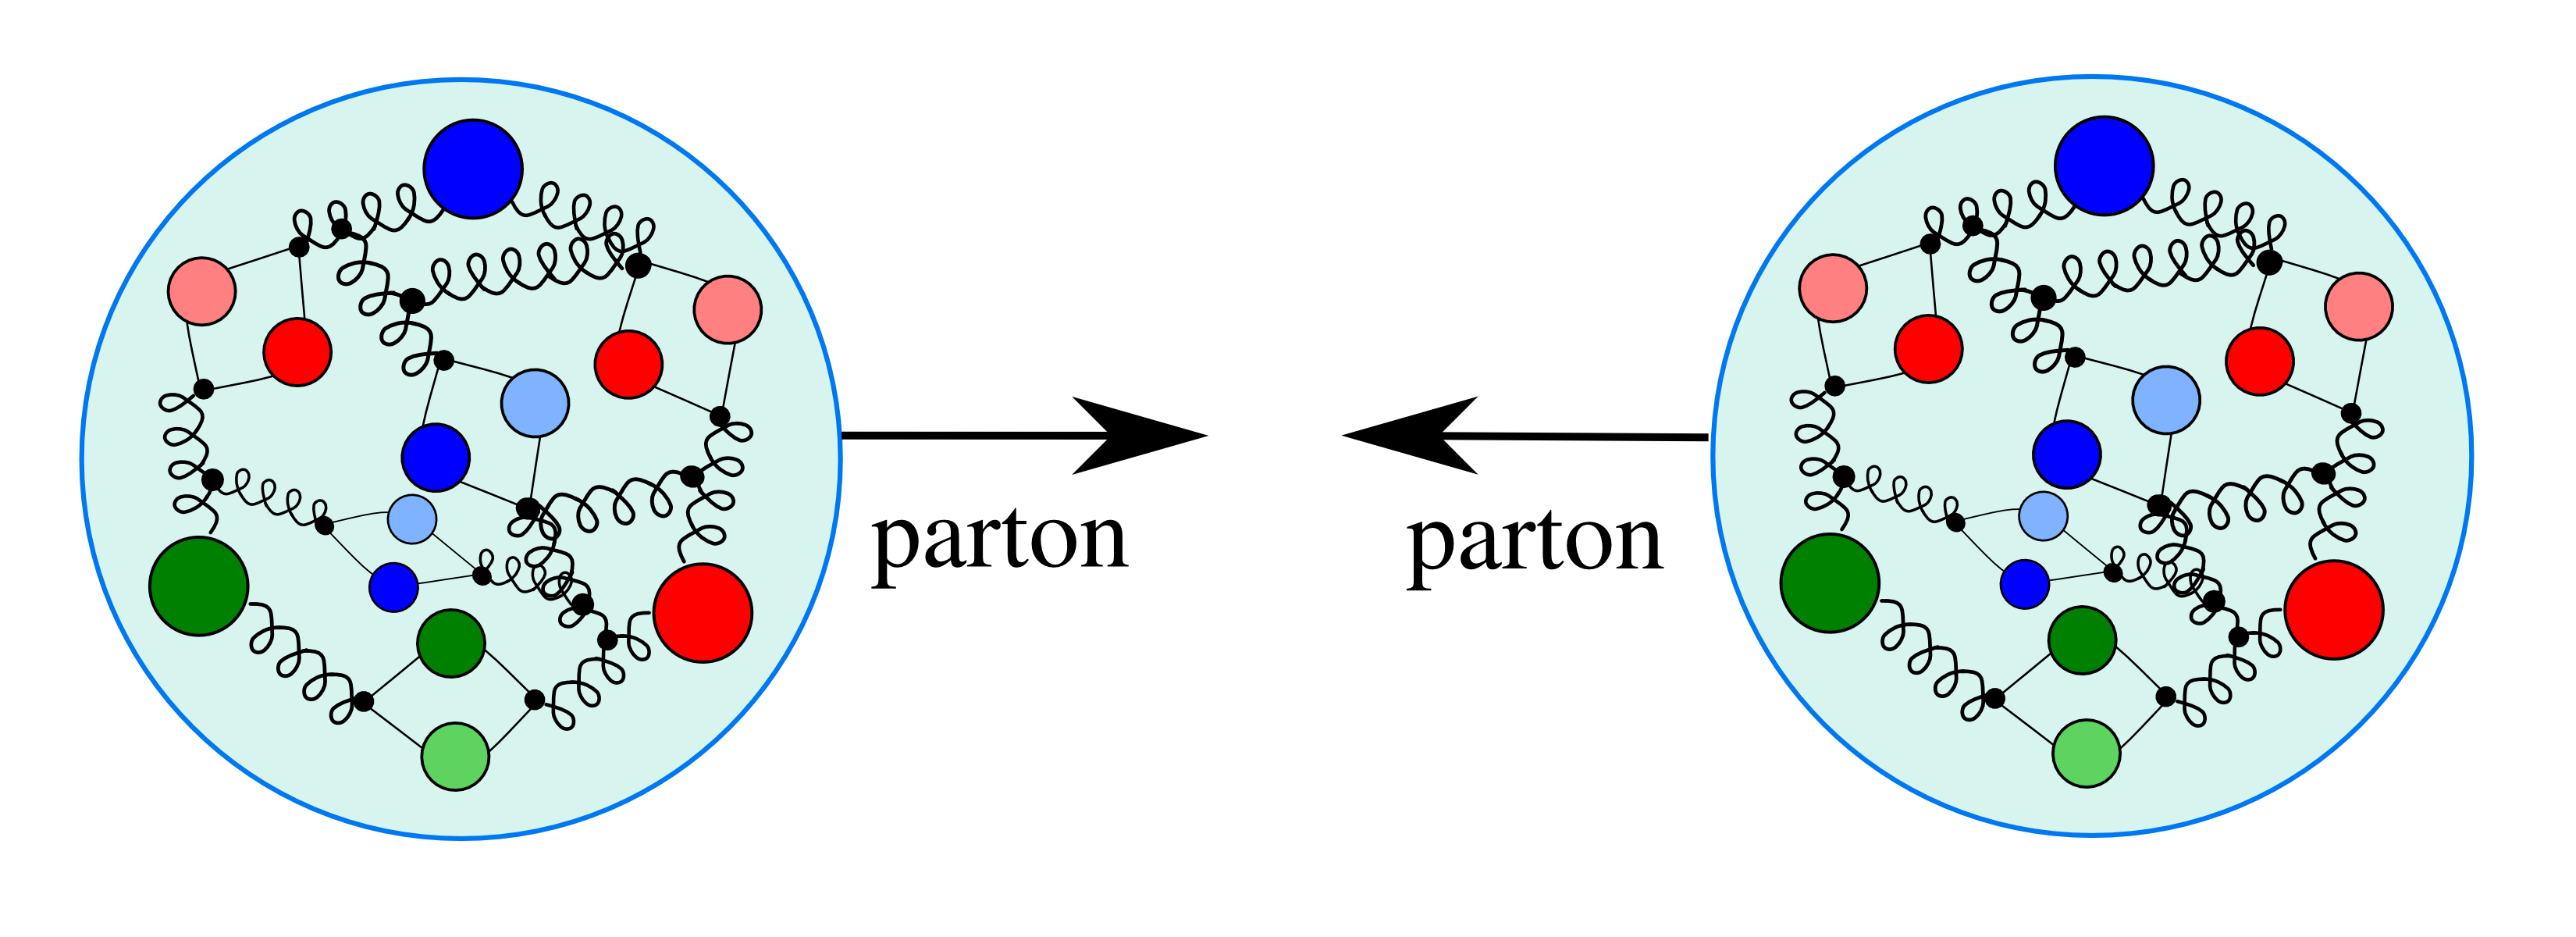
\includegraphics[width=0.45\textwidth]{../figs/Intro/ppCollision.png}}
    \caption{The proton structure (left) and the proton-proton collision (right).}
    \label{fig:ppCollision}
  \end{center}
\end{figure}

